Adesso vediamo le proprietà dei quark e dei gluoni da un altro punto di vista. 
\subsection{Esperimento di scattering}
\begin{itemize}
    \item Vogliamo sapere se il bersaglio è un semplice oggetto puntiforme, e se non lo è dobbiamo capire come sondare la sua struttura. 
    \item Per fare ciò ci serviamo di esperimenti di scattering. Potremmo fare scattering di Rutherford (1911) ma utilizzò particelle $\alpha$ e non riusci neanche a vedere la dimensione del nucleo (di oro). Infatti successivamente tra 1950-1960 Hofstadter arrivò alla struttura nucleare con elettroni in nuclei di $H/D/He$ e infine tra 1965-1980 (SLAC/CERN) con elettroni siamo arrivati alla materia adronica cioè i quark.
    \item Usiamo come sonda una particella elementare, normalmente un elettrone, perché oltre ad essere semplici da produrre, vogliamo essere in grado di scegliere noi la energia della sonda e soprattutto perché così siamo "sicuri" che il proiettile sia elementare e tutti gli effetti di non-elementarietà sono dovuti esclusivamente al bersaglio.
    \item Dunque in ordine:
    \begin{enumerate}
        \item Si sceglie una sonda (e.g. elettrone)
        \item Si studia lo scattering $e^-$-target 
        \item Si misura la sezione d'urto di $e^-T$, la distribuzione angolare di $e^-$ e si rivelano stati eccitati o lo stato finale del sistema adronico (scattering anelastico)
    \end{enumerate}
    \item Il modo di procedere è:
    \begin{enumerate}
        \item Si studia la cinematica. Con cinematica intendiamo le equazioni che seguono dalla conservazione di momento angolare e massa. Dopo aver imposto i vincoli cinematici si studia la \textit{dinamica}. 
        \item Calcoliamo la $\sigma(e^-T)$ per nuclei puntuali in elettrodinamica classica (formula di Rutherford).
        \item Si fa lo stesso per la meccanica quantistica con elettroni ($s=\frac12$) e nuclei puntuali (formula di Mott)
        \item Si rivelano \textit{deviazioni} da questi modelli. Così derivo informazioni sulla struttura nucleare
        \item Formulo una nuova teoria, poi vado a distanze ancora più piccole ($Q^2$ maggiore) e vedo se la nuova teoria regge o ci sono altre deviazioni e ripeto, potenzialmente fino all'infinito.
    \end{enumerate}
\end{itemize}
\begin{figure}[H]
    \centering
    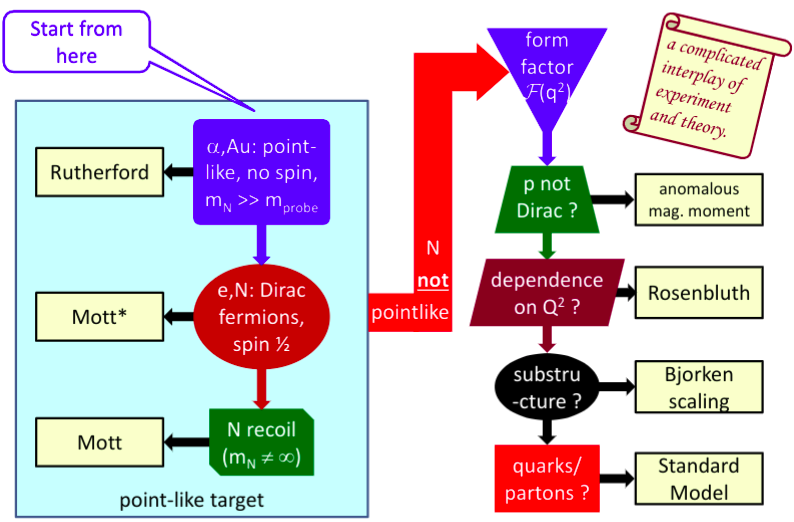
\includegraphics[width=0.7\textwidth]{immagini/fig_treasure_map_scattering}
    \caption{Mappa del tesoro dello scattering.}
    %\label{}
\end{figure}
\subsection{Modello a gas di Fermi}
\begin{itemize}
    \item I nuclei sono stati legati di protoni e neutroni. Il gas di Fermi è un semplice modello.
    \item I protoni e i neutroni sono identici a meno della carica: sono delle sfere con una certa massa; sono fermioni; sono legati all'interno del nucleo, altrimenti sono liberi di muoversi. 
    \item Non consideriamo interazione elettromagnetica, solo nucleare dunque $N=Z=\frac A2$ ed impulso ed energia di Fermi sono uguali per protoni e neutroni (in approssimazione migliore sono differenti gli impulsi). 
    \item Per il principio di indeterminazione ogni $p$ ed $n$ occupano un volume $V=(2\pi\hbar)3$ nello spazio delle fasi.
    \item Dunque abbiamo una buca ben definita identica per protoni e neutroni, e viene rispettata la statistica di Fermi dunque due $p/n$ per livello di energia (con spin opposto).
    \item Da queste approssimazioni possiamo fare dei calcoli semplici:
    \begin{gather*}
    n_n^\uparrow=n_n^\downarrow=n_p^\uparrow=n_p^\downarrow=\frac N2=\frac Z2=\frac A4=\\
    =\frac{[V\_{space}V\_{imp}]\_{TOT}}{[V\_{space}V\_{imp}]\_{ciascuna particella}}=\frac{\frac43\pi r_0^3A\times\frac43\pi p_F^3}{(2\pi\hbar)^3}=\frac{2Ar_0^3p_F^3}{9\pi^2\hbar^3}\implies\\
    \implies N=Z=\frac A2=\frac{4Ar_0^3p_F^3}{9\pi^2\hbar^3}\implies p_F=\frac\hbar{r_0}\sqrt[3]{\frac{9\pi}8}\underset{r_0\approx1.2\,\text{fm}}{\implies}
    \begin{cases}
    p_F\approx250\,\MeV\\
    E_F^{\text{kin}}=\frac{p_F^2}{2m}\approx33\,\MeV
    \end{cases}
    \end{gather*}
    dove il valore di $r_0$ viene da fit del fattore di forma (vedi dopo) e per $E^{\text{kin}}_F$ si è considerata approssimazione non relativistica. 
    \item In conclusione
\end{itemize}